\chapter{Algebra and Equations}
\label{chap:III_algebra}

Mathematics begins not only with numbers, but also with relationships.
As soon as one no longer merely counts, but wants to describe a connection,
a new form of thinking appears:
\emph{algebra}\index{algebra}.

While numbers express individual quantities or magnitudes,
algebra asks about the general.
It examines how quantities are connected with one another,
how the unknown can be determined from the known,
and how concrete problems become general structures.

Algebra thus marks a decisive step
in the development of mathematics:
it detaches itself from the individual calculation
and becomes a language of relationships, rules, and forms.
In this sense, \emph{equations}\index{equation}
are not merely calculation problems,
but precise statements about relationships.

This chapter shows
how a general method arose from practical problems,
how equations became tools of mathematical thinking,
and why algebra is far more
than calculating with letters.

% =====================================================
% 3.1 Arabic Mathematics and the Birth of Algebra
% =====================================================
\subsection{Arabic Mathematics and the Birth of Algebra}
\label{sec:3.1_arabic_mathematics}

After the Greeks\index{Greeks}, Indians\index{India}, and Babylonians\index{Babylonia},
it was the Arabic-Islamic world\index{Arabic mathematics}
that raised mathematics\index{mathematics} to a new, systematic level.
While in Europe\index{Europe} much of ancient knowledge survived only in fragments,
scholars such as
\emph{al-Khwarizmi}\index{al-Khwarizmi, Muhammad ibn Musa},
\emph{Omar Khayyam}\index{Khayyam, Omar}, and
\emph{al-Karaji}\index{al-Karaji, Abu Bakr}
preserved, translated, and expanded the insights of their predecessors.

In the ninth century, \emph{al-Khwarizmi} wrote in Baghdad\index{Baghdad}
the work
\emph{Kitāb al-jabr wa’l-muqābala}\index{Kitāb al-jabr wa’l-muqābala},
which is regarded as the birth of \emph{algebra}\index{algebra}.
The term ``al-jabr'' roughly means ``restoration'' or ``completion,''
while ``al-muqābala'' means ``balancing'' or ``setting against.''
What was meant was a method for isolating the unknown\index{unknown}
and systematically simplifying equations\index{equations}.
This marked the beginning of a new stage in mathematics:
the focus was no longer only on individual numbers or geometric figures,
but on general relationships between quantities.

\begin{HistoryBox}[From Practice to Theory]
	\phantomsection\label{box:practice}
	Arabic mathematics initially centered on practical problems:
	the distribution of inheritances, the calculation of land areas,
	the determination of trade shares, or astronomical measurements\index{astronomy}.
	From such concrete tasks, however, a general method developed
	for systematically determining unknown quantities.
	This is the true origin of algebra.
\end{HistoryBox}

A classic example from this context is the calculation of inheritance shares\index{inheritance share}.
According to Islamic law\index{Islamic law}, a wife receives one eighth of the estate,
and the remainder is divided equally among the sons.
If the total inheritance amounts to 600~dinars, then one obtains:
\[
600 = \tfrac{1}{8}\cdot 600 + 2x.
\]

The wife receives
\[
\frac{1}{8}\cdot 600 = 75,
\]
so for the two sons there remain
\[
600 - 75 = 525.
\]
Thus each son receives
\[
x = \frac{525}{2} = 262{,}5 \text{ dinars}.
\]

\begin{HistoryBox}[From Practical Problem to Abstract Equation]
	\phantomsection\label{box:abstractequation}
	The decisive step of algebra consisted in translating
	a concrete situation into a general form.
	The inheritance problem is no longer merely described in words,
	but formulated as an equation:
	\[
	600 = \frac{1}{8}\cdot 600 + 2x.
	\]
	In this way, a practical question becomes a mathematical problem
	that can be solved by fixed rules.
\end{HistoryBox}

\begin{NoteBox}[A Shared Heritage]
	\phantomsection\label{box:heritage}
	The Arabic mathematicians did not invent algebra out of nothing.
	They built on the knowledge of the Babylonians, Greeks, and Indians.
	The Babylonians had already solved equations of the form \(x^2 + bx = c\)
	using tabular methods; the Greeks described geometric relationships
	that were algebraic at their core;
	and in India, symbolic methods of calculation with unknowns emerged
	(\emph{yāvattavat}).
	The achievement of the Arabic scholars consisted in connecting these traditions,
	ordering them, and developing them into a coherent method.
\end{NoteBox}

% =====================================================
% 3.2 Al-Khwarizmi: Completing the Square as an Area Argument
% =====================================================
\subsection{Al-Khwarizmi: Completing the Square as an Area Argument}

A well-known example from al-Khwarizmi's work reads:
\begin{quote}
	``A square and ten of its roots amount to thirty-nine.''
\end{quote}
Today we write this as the equation
\[
x^2 + 10x = 39.
\]

Al-Khwarizmi thought geometrically:
\(x^2\) is the area of a square with side length \(x\),
and the term \(10x\) can also be interpreted as an area.

\vspace{0.6em}

\begin{figure}[htbp]
	\centering
	
	\begin{subfigure}[t]{0.32\linewidth}
		\centering
		\includegraphics[width=\linewidth]{bilder/alch02.png}
		\caption{Areas: \(x^2\) and \(10x\).}
		\label{fig:alch02}
	\end{subfigure}\hfill
	\begin{subfigure}[t]{0.32\linewidth}
		\centering
		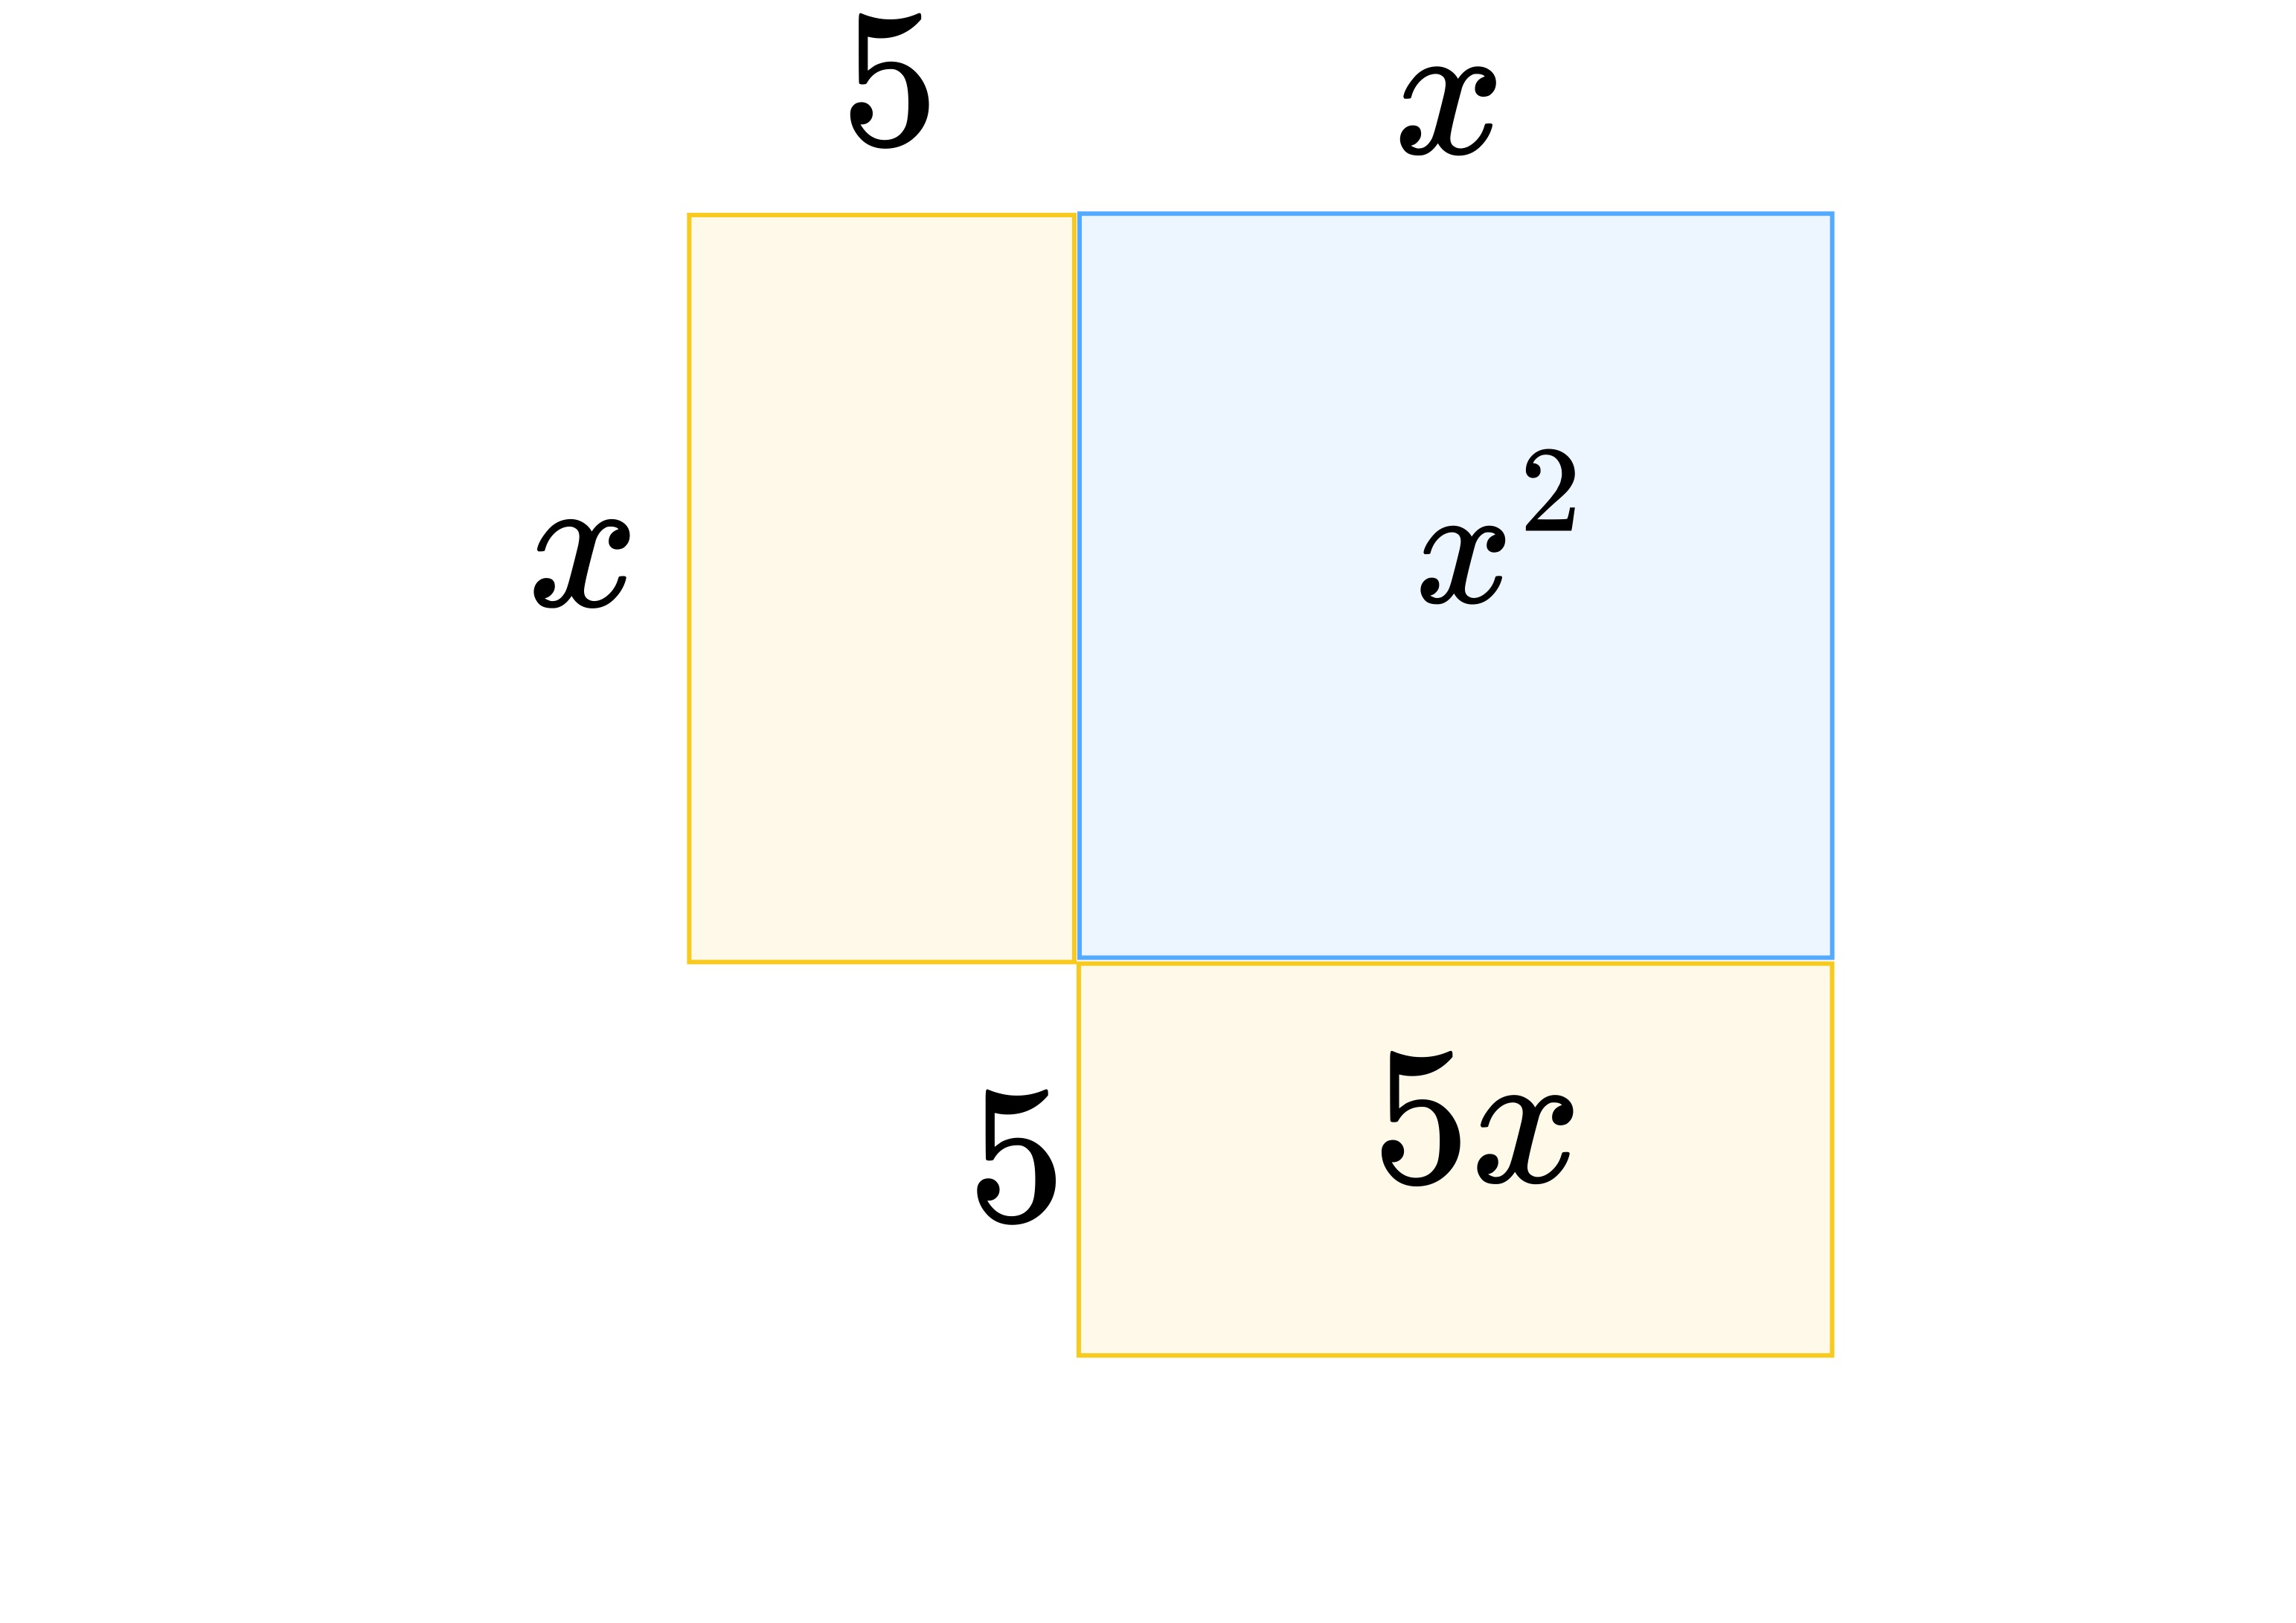
\includegraphics[width=\linewidth]{bilder/alch01.png}
		\caption{Decomposition: \(10x=2\cdot 5x\).}
		\label{fig:alch01}
	\end{subfigure}\hfill
	\begin{subfigure}[t]{0.32\linewidth}
		\centering
		\includegraphics[width=\linewidth]{bilder/alch03.png}
		\caption{\(+25\Rightarrow (x+5)^2\).}
		\label{fig:alch03}
	\end{subfigure}
	
	\caption{Completing the square according to al-Khwarizmi as an area argument.}
	\label{fig:alchwarizmi}
\end{figure}

The term \(10x\) is decomposed as
\[
10x = 5x + 5x,
\]
that is, into two rectangles of size \(x\times 5\),
which are placed along two sides of the square.
This almost creates a larger square;
only the corner square \(5\times 5\), with area \(25\), is still missing.

If this missing area is added to both sides, one obtains
\[
x^2 + 10x + 25 = 39 + 25,
\]
and therefore
\[
(x+5)^2 = 64.
\]
Geometrically, this means:
the completed square has area \(64\) and therefore side length \(8\).
Since lengths are being considered here, only the positive solution is relevant.
Thus
\[
x+5 = 8
\]
and therefore
\[
x = 3.
\]

\begin{DidacticBox}[The Origin of the Word ``Algorithm'']
	\phantomsection\label{box:origin}
	The name \emph{al-Khwarizmi} was transformed in Latin into ``Algoritmi.''
	From this came the word \emph{algorithm}\index{algorithm}.
	Thus the idea of rule-based, step-by-step calculation\index{calculation}
	also goes back to Arabic science.
\end{DidacticBox}

Algebra was therefore not simply a new collection of calculation tricks,
but a reorganization of mathematical knowledge.
It connected arithmetic, geometry, and methods of transformation
into a general language of relationships.
Precisely there lies its true significance.

% =====================================================
% 3.3 Equations as Tools for Solving Problems
% =====================================================

\subsection{Equations as Tools for Solving Problems}
\label{sec:3.2_equations}
\phantomsection

\subsubsection*{Introduction}
\phantomsection
Since antiquity\index{antiquity}, tasks repeatedly appeared in trade\index{trade},
geometry\index{geometry}, and astronomy\index{astronomy}
in which an unknown quantity\index{unknown}
had to be determined.
At first this was done with words, tables, or geometric constructions.
Only gradually did this develop into a method
that fundamentally simplified dealing with the unknown:
the \emph{equation}\index{equation}.

An equation makes a problem not only calculable,
but also generally formulable.
It translates a concrete situation into a form
that can be handled according to fixed rules.

\subsubsection*{From Sentence to Equation}
\phantomsection
Early equations usually arose from word problems:
a merchant sells part of his goods,
a field has an unknown side length,
or an astronomical relationship requires an unknown quantity.
Such situations were initially described in words.
Only later did symbolic notation become established.

The decisive advance consisted in the fact
that an equation was no longer understood merely as a calculation aid,
but as the expression of a relationship.
It states that two expressions have the same value.
Whoever understands this relationship
can systematically determine unknown quantities.

\subsubsection*{Equations as a Universal Tool}
\phantomsection
With \emph{algebra}\index{algebra}, a new approach to problems emerged:

\begin{itemize}
	\item Geometric relationships could be formulated algebraically.
	\item Trade and interest calculations\index{interest calculation} could be expressed as linear equations\index{linear equation}.
	\item Areas and volumes led to quadratic\index{quadratic equation} and cubic equations\index{cubic equation}.
	\item Problems of motion became equations in time\index{equation of motion}.
\end{itemize}

In this way, the equation became a universal tool.
Not every problem had to be solved individually anymore;
what mattered now was recognizing its structure
and translating it into a suitable equation.

\subsubsection*{Equations and the Expanded Concept of Number}
\phantomsection
The history of equations also shows something deeper:
equations do not merely find solutions;
at times, they also force new domains of numbers to emerge.

Quadratic equations led to expressions
that could not be treated meaningfully without irrational or negative numbers.
Cubic equations, in certain solution procedures, even led to terms such as \(\sqrt{-1}\)
and thus opened the way to the complex numbers\index{complex numbers}.

This contains a fundamental idea:
\medskip

\textit{Algebra shows which numbers must exist
	in order for its equations to become solvable.}

\medskip

\subsubsection*{A Real-World Example}
\phantomsection
A simple everyday problem shows this way of thinking particularly clearly.
A water tank loses 3 liters of water per minute
through a small leak.
At the beginning it contains 20 liters.
When is the tank empty?

The situation can be written directly as an equation:
\[
20 - 3t = 0.
\]

By rearranging, one obtains
\[
t = \frac{20}{3} \approx \SI{6.7}{\minute}.
\]

The example is simple,
but the structure is general.
A real situation is formalized\index{formalization},
and precisely through this it becomes calculable.

\begin{DidacticBox}[Why Equations Represent Reality]
	\phantomsection\label{box:reality}
	In many everyday situations, an equation arises quite naturally.
	It gathers the essential quantities
	and makes their relationship calculable.
	
	In the case of the leaking water tank,
	\[
	20 - 3t = 0
	\]
	the structure of the problem forces the equation.
	For this reason, equations are not merely calculation aids,
	but general tools for describing real relationships.
\end{DidacticBox}

\subsubsection*{Transition}
\phantomsection
At this point, a second achievement of algebra becomes visible.
It not only helps solve individual problems,
but turns concrete tasks into general forms.
Precisely here the step from practical calculation
to structural thinking becomes clear.

% =====================================================
% 3.4 From the Concrete Problem to the General Form
% =====================================================

\subsection{From the Concrete Problem to the General Form}
\label{sec:3.4_general_form}
\phantomsection

\subsubsection*{Introduction}
\phantomsection
The true strength of algebra lies not only
in solving individual tasks.
What is decisive, rather,
is that it derives general forms from concrete problems.
An inheritance case, a trade calculation, or an area problem
may at first seem very different.
Algebraically, however, they can possess the same structure.

\subsubsection*{The General in the Particular}
\phantomsection
A concrete problem usually contains numbers,
a factual relationship, and a quantity being sought.
Algebra detaches itself from this external framework
and concentrates on the relationship between the quantities.

Thus a story about possession, shares, or lengths
becomes an equation.
The individual case is no longer at the center;
instead, the pattern visible within it becomes decisive.

\subsubsection*{Why Letters Are More Than Placeholders}
\phantomsection
The introduction of symbols such as \(x\) or \(y\)
is therefore far more than an abbreviation.
A letter does not merely stand for an unknown number,
but for a position within a general structure.

The equation
\[
ax+b=0
\]
is not a single problem,
but the form of all linear equations of this type.
Whoever understands this form
also understands infinitely many concrete problems.

\subsubsection*{From Example to Form}
\phantomsection
An individual problem is often the starting point,
but not the true goal of algebra.
What matters is
that behind a concrete example
a general form can be recognized.

Thus an inheritance problem becomes a linear equation,
and an area problem becomes a quadratic equation.
The individual numbers can change,
but the underlying structure remains the same.
Precisely this makes mathematics transferable and general.

\subsubsection*{Algebra as Generalization}
\phantomsection
This is the progress achieved by algebra:
it frees calculation from the individual case.
Instead of treating each problem anew,
it recognizes common patterns
and develops methods
that can be applied to many situations at once.

Mathematics thereby becomes not only more practical,
but also deeper.
It no longer merely describes individual results,
but general relationships.

\begin{DidacticBox}[What Algebra Really Does]
	\phantomsection\label{box:generalform}
	Algebra does not simply mean
	calculating with letters instead of numbers.
	Its true achievement consists in recognizing
	the general within the particular.
	
	An equation therefore never stands only for an individual case,
	but for a structure
	that recurs in many different problems.
\end{DidacticBox}

\subsubsection*{Transition}
\phantomsection
As soon as mathematics is understood as a system of general forms,
the next question arises:
Why do these forms work so reliably?
This brings the role of rules and axioms into focus.

% =====================================================
% 3.5 Mathematics as a System of Rules
% =====================================================

\subsection{Mathematics as a System of Rules}
\label{sec:3.5_system_of_rules}
\phantomsection

\subsubsection*{Introduction}
\phantomsection
The developments so far -- from the first methods of solving equations
to the general symbolic form --
show a central pattern:
\emph{mathematics}\index{mathematics}
does not grow through arbitrary ideas,
but through the inner logic of its rules\index{rules}.
Once fixed rules of calculation are accepted,
new structures\index{structure} often follow inevitably.

Mathematics is therefore not a collection of isolated tricks,
but a coherent system.

\subsubsection*{Rules as the Basis of Mathematical Thinking}
\phantomsection
Since antiquity\index{antiquity},
mathematical thinking has been based on fixed operations:
addition\index{addition}, subtraction\index{subtraction},
multiplication\index{multiplication}, and division\index{division}.
Every extension of the concept of number\index{concept of number}
could establish itself only if these rules remained consistent.

This applies to
\begin{itemize}
	\item the introduction of zero\index{zero},
	\item the acceptance of negative numbers,
	\item the insight into the irrationality of $\sqrt{2}$\index{irrational numbers},
	\item the complex numbers \(a+bi\),
	\item and later structures such as vectors\index{vector} or functions\index{function}.
\end{itemize}

The decisive point is:
once the rules are clearly established,
their consequences must be taken seriously --
even if they at first seem unfamiliar.

\subsubsection*{The Idea of Axioms}
\phantomsection
A system of rules is viable only
if it is based on clear fundamental assumptions.
Such fundamental assumptions are called \emph{axioms}\index{axiom}.
They determine
how mathematical objects may be connected with one another
without producing contradictions.

For the complex numbers, only a few specifications are sufficient:
\begin{itemize}
	\item \(i^2 = -1\)\index{$i^2=-1$},
	\item real and imaginary parts are added componentwise,
	\item the familiar rules of calculation are continued consistently.
\end{itemize}

From such specifications, a complete domain of numbers\index{number domain} emerges.
Axioms do not restrict mathematics --
they make its structure possible in the first place.

\subsubsection*{Systems of Rules Generate Mathematical Worlds}
\phantomsection
Once the rules are fixed,
one can investigate
which objects and relationships exist within this system.
In this way, mathematical worlds with their own inner order arise.

\begin{itemize}
	\item From arithmetic\index{arithmetic} develop the natural\index{natural numbers}, integer\index{integers}, and rational numbers\index{rational numbers}.
	\item From geometric axioms arises Euclidean geometry\index{Euclidean geometry}.
	\item From the field axioms\index{field axioms} develops analysis\index{analysis}.
	\item From the rules of algebra\index{algebra} arise polynomial equations\index{polynomial equation} and their solution structures.
\end{itemize}

Mathematics thus develops, in a certain sense, from within.
It is not constructed arbitrarily,
but unfolded from clear assumptions.

\begin{DidacticBox}[Why Rules Carry Mathematics]
	\phantomsection\label{box:rules}
	Mathematics often appears like a collection of separate topics:
	numbers, equations, functions, or geometry.
	In fact, these areas are connected
	because they are based on a few fundamental rules.
	
	Once these rules are fixed,
	many structures follow not from arbitrariness,
	but from consequence.
	For this reason, new domains of numbers are not simply invented,
	but recognized as necessary.
\end{DidacticBox}

\subsubsection*{Mathematics Is Not Invented, but Discovered}
\phantomsection
The history of numbers\index{numbers} and algebra\index{algebra}
therefore shows a clear pattern:
new structures do not arise
because one freely wants to invent them,
but because the existing rules suggest them or even force them.
Negative numbers, irrational numbers, and complex numbers
are not products of mere imagination,
but consequences of mathematical structure.

\subsubsection*{Transition}
\phantomsection
If mathematical rules generate a consistent world,
the next question almost arises by itself:
Why does this world so often reflect the structure of nature?
This connection leads into the following chapter.